% shanghai q17 fig1: regular square pyramid P-ABCD, O center
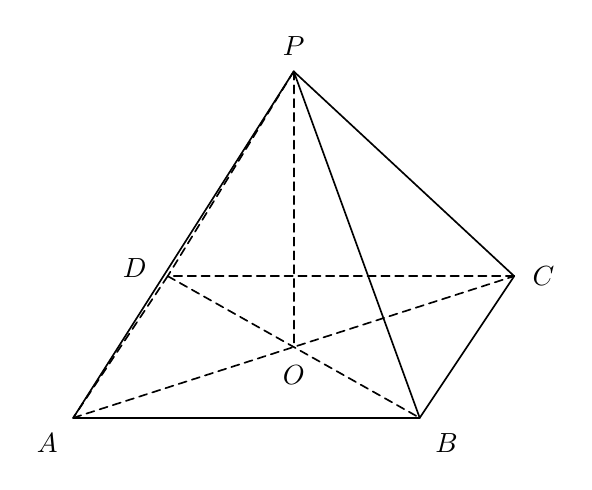
\begin{tikzpicture}[line width=.6pt, line join=round, line cap=round]
\coordinate (P) at (2.8000000000,4.4000000000);
\coordinate (A) at (0,0);
\coordinate (B) at (4.4,0);
\coordinate (C) at (5.6,1.8);
\coordinate (D) at (1.2,1.8);
\coordinate (O) at (2.8000000000,0.9000000000);
% base
\draw[solid] (A) -- (B);
\draw[solid] (B) -- (C);
\draw[densely dashed] (C) -- (D);
\draw[densely dashed] (D) -- (A);
\draw[densely dashed] (A) -- (C);
\draw[densely dashed] (D) -- (B);
% lateral
\draw[solid] (P) -- (A);
\draw[solid] (P) -- (B);
\draw[solid] (P) -- (C);
\draw[densely dashed] (P) -- (D);
\draw[densely dashed] (P) -- (O);
% base diagonals mark O


\node[above=2pt] at (P) {$P$};
\node[below left=2pt] at (A) {$A$};
\node[below right=2pt] at (B) {$B$};
\node[right=3pt] at (C) {$C$};
\node[left=3pt,xshift=-1pt,yshift=3pt] at (D) {$D$};
\node[below=3pt] at (O) {$O$};
\end{tikzpicture}
